%-----------------------------------------------------------------------------------------------------------------------------------------------%
%	The MIT License (MIT)
%
%	Copyright (c) 2019 Jan Küster
%
%	Permission is hereby granted, free of charge, to any person obtaining a copy
%	of this software and associated documentation files (the "Software"), to deal
%	in the Software without restriction, including without limitation the rights
%	to use, copy, modify, merge, publish, distribute, sublicense, and/or sell
%	copies of the Software, and to permit persons to whom the Software is
%	furnished to do so, subject to the following conditions:
%	
%	THE SOFTWARE IS PROVIDED "AS IS", WITHOUT WARRANTY OF ANY KIND, EXPRESS OR
%	IMPLIED, INCLUDING BUT NOT LIMITED TO THE WARRANTIES OF MERCHANTABILITY,
%	FITNESS FOR A PARTICULAR PURPOSE AND NONINFRINGEMENT. IN NO EVENT SHALL THE
%	AUTHORS OR COPYRIGHT HOLDERS BE LIABLE FOR ANY CLAIM, DAMAGES OR OTHER
%	LIABILITY, WHETHER IN AN ACTION OF CONTRACT, TORT OR OTHERWISE, ARISING FROM,
%	OUT OF OR IN CONNECTION WITH THE SOFTWARE OR THE USE OR OTHER DEALINGS IN
%	THE SOFTWARE.
%	
%
%-----------------------------------------------------------------------------------------------------------------------------------------------%


%============================================================================%
%
%	DOCUMENT DEFINITION
%
%============================================================================%

%we use article class because we want to fully customize the page and don't use a cv template
\documentclass[10pt,A4]{article}	


%----------------------------------------------------------------------------------------
%	ENCODING
%----------------------------------------------------------------------------------------

% we use utf8 since we want to build from any machine
\usepackage[utf8]{inputenc}		

%----------------------------------------------------------------------------------------
%	LOGIC
%----------------------------------------------------------------------------------------

% provides \isempty test
\usepackage{xstring, xifthen}

%----------------------------------------------------------------------------------------
%	FONT BASICS
%----------------------------------------------------------------------------------------

% some tex-live fonts - choose your own

%\usepackage[defaultsans]{droidsans}
%\usepackage[default]{comfortaa}
%\usepackage{cmbright}
\usepackage[default]{raleway}
%\usepackage{fetamont}
%\usepackage[default]{gillius}
%\usepackage[light,math]{iwona}
%\usepackage[thin]{roboto} 

% set font default
\renewcommand*\familydefault{\sfdefault} 	
\usepackage[T1]{fontenc}

% more font size definitions
\usepackage{moresize}

%----------------------------------------------------------------------------------------
%	FONT AWESOME ICONS
%---------------------------------------------------------------------------------------- 

% include the fontawesome icon set
\usepackage{fontawesome}

% use to vertically center content
% credits to: http://tex.stackexchange.com/questions/7219/how-to-vertically-center-two-images-next-to-each-other
\newcommand{\vcenteredinclude}[1]{\begingroup
\setbox0=\hbox{\includegraphics{#1}}%
\parbox{\wd0}{\box0}\endgroup}

% use to vertically center content
% credits to: http://tex.stackexchange.com/questions/7219/how-to-vertically-center-two-images-next-to-each-other
\newcommand*{\vcenteredhbox}[1]{\begingroup
\setbox0=\hbox{#1}\parbox{\wd0}{\box0}\endgroup}

% icon shortcut
\newcommand{\icon}[3] { 							
	\makebox(#2, #2){\textcolor{maincol}{\csname fa#1\endcsname}}
}	

% icon with text shortcut
\newcommand{\icontext}[4]{ 						
	\vcenteredhbox{\icon{#1}{#2}{#3}}  \hspace{2pt}  \parbox{0.9\mpwidth}{\textcolor{#4}{#3}}
}

% icon with website url
\newcommand{\iconhref}[5]{ 						
    \vcenteredhbox{\icon{#1}{#2}{#5}}  \hspace{2pt} \href{#4}{\textcolor{#5}{#3}}
}

% icon with email link
\newcommand{\iconemail}[5]{ 						
    \vcenteredhbox{\icon{#1}{#2}{#5}}  \hspace{2pt} \href{mailto:#4}{\textcolor{#5}{#3}}
}

%----------------------------------------------------------------------------------------
%	PAGE LAYOUT  DEFINITIONS
%----------------------------------------------------------------------------------------

% page outer frames (debug-only)
% \usepackage{showframe}		

% we use paracol to display breakable two columns
\usepackage{paracol}

% define page styles using geometry
\usepackage[a4paper]{geometry}

% remove all possible margins
\geometry{top=1cm, bottom=1cm, left=1cm, right=1cm}

\usepackage{fancyhdr}
\pagestyle{empty}

% space between header and content
% \setlength{\headheight}{0pt}

% indentation is zero
\setlength{\parindent}{0mm}

%----------------------------------------------------------------------------------------
%	TABLE /ARRAY DEFINITIONS
%---------------------------------------------------------------------------------------- 

% extended aligning of tabular cells
\usepackage{array}

% custom column right-align with fixed width
% use like p{size} but via x{size}
\newcolumntype{x}[1]{%
>{\raggedleft\hspace{0pt}}p{#1}}%


%----------------------------------------------------------------------------------------
%	GRAPHICS DEFINITIONS
%---------------------------------------------------------------------------------------- 

%for header image
\usepackage{graphicx}

% use this for floating figures
% \usepackage{wrapfig}
% \usepackage{float}
% \floatstyle{boxed} 
% \restylefloat{figure}

%for drawing graphics		
\usepackage{tikz}				
\usetikzlibrary{shapes, backgrounds,mindmap, trees}

%----------------------------------------------------------------------------------------
%	Color DEFINITIONS
%---------------------------------------------------------------------------------------- 
\usepackage{transparent}
\usepackage{color}

% primary color
\definecolor{maincol}{RGB}{0, 158, 97}

% accent color, secondary
% \definecolor{accentcol}{RGB}{ 250, 150, 10 }

% dark color
\definecolor{darkcol}{RGB}{0.0, 158, 97}

% light color
\definecolor{lightcol}{RGB}{197, 237, 221}


% Package for links, must be the last package used
\usepackage[hidelinks]{hyperref}

% returns minipage width minus two times \fboxsep
% to keep padding included in width calculations
% can also be used for other boxes / environments
\newcommand{\mpwidth}{\linewidth-\fboxsep-\fboxsep}
	


%============================================================================%
%
%	CV COMMANDS
%
%============================================================================%

%----------------------------------------------------------------------------------------
%	 CV LIST
%----------------------------------------------------------------------------------------

% renders a standard latex list but abstracts away the environment definition (begin/end)
\newcommand{\cvlist}[1] {
	\begin{itemize}{#1}\end{itemize}
}

%----------------------------------------------------------------------------------------
%	 CV TEXT
%----------------------------------------------------------------------------------------

% base class to wrap any text based stuff here. Renders like a paragraph.
% Allows complex commands to be passed, too.
% param 1: *any
\newcommand{\cvtext}[1] {
	\begin{tabular*}{1\mpwidth}{p{0.98\mpwidth}}
		\parbox{1\mpwidth}{#1}
	\end{tabular*}
}

%----------------------------------------------------------------------------------------
%	CV SECTION
%----------------------------------------------------------------------------------------

% Renders a a CV section headline with a nice underline in main color.
% param 1: section title
\newcommand{\cvsection}[1] {
	\vspace{14pt}
	\cvtext{
		\textbf{\LARGE{\textcolor{darkcol}{\uppercase{#1}}}}\\[-4pt]
		\textcolor{maincol}{ \rule{0.1\textwidth}{2pt} } \\
	}
}

%----------------------------------------------------------------------------------------
%	META SKILL
%----------------------------------------------------------------------------------------

% Renders a progress-bar to indicate a certain skill in percent.
% param 1: name of the skill / tech / etc.
% param 2: level (for example in years)
% param 3: percent, values range from 0 to 1
\newcommand{\cvskill}[3] {
	\begin{tabular*}{1\mpwidth}{p{0.72\mpwidth}  r}
 		\textcolor{black}{\textbf{#1}} & \textcolor{maincol}{#2}\\
	\end{tabular*}%
	
	\hspace{4pt}
	\begin{tikzpicture}[scale=1,rounded corners=2pt,very thin]
		\fill [lightcol] (0,0) rectangle (1\mpwidth, 0.15);
		\fill [maincol] (0,0) rectangle (#3\mpwidth, 0.15);
  	\end{tikzpicture}%
}


%----------------------------------------------------------------------------------------
%	 CV EVENT
%----------------------------------------------------------------------------------------

% Renders a table and a paragraph (cvtext) wrapped in a parbox (to ensure minimum content
% is glued together when a pagebreak appears).
% Additional Information can be passed in text or list form (or other environments).
% the work you did
% param 1: time-frame i.e. Sep 14 - Jan 15 etc.
% param 2:	 event name (job position etc.)
% param 3: Customer, Employer, Industry
% param 4: Short description
% param 5: work done (optional)
% param 6: technologies include (optional)
% param 7: achievements (optional)
\newcommand{\cvevent}[7] {
	
	% we wrap this part in a parbox, so title and description are not separated on a pagebreak
	% if you need more control on page breaks, remove the parbox
	\parbox{\mpwidth}{
		\begin{tabular*}{1\mpwidth}{p{0.72\mpwidth}  r}
	 		\textcolor{black}{\textbf{#2}} & \colorbox{maincol}{\makebox[0.25\mpwidth]{\textcolor{white}{#1}}} \\
			\textcolor{maincol}{\textbf{#3}} & \\
		\end{tabular*}\\[8pt]
	
		\ifthenelse{\isempty{#4}}{}{
			\cvtext{#4}\\
		}
	}

	\ifthenelse{\isempty{#5}}{}{
		\vspace{9pt}
		{#5}
	}

	\ifthenelse{\isempty{#6}}{}{
		\vspace{9pt}
		\cvtext{\textbf{Technologies include:}}\\
		{#6}
	}

	\ifthenelse{\isempty{#7}}{}{
		\vspace{9pt}
		\cvtext{\textbf{Achievements include:}}\\
		{#7}
	}
	\vspace{14pt}
}

%----------------------------------------------------------------------------------------
%	 CV META EVENT
%----------------------------------------------------------------------------------------

% Renders a CV event on the sidebar
% param 1: title
% param 2: subtitle (optional)
% param 3: customer, employer, etc,. (optional)
% param 4: info text (optional)
\newcommand{\cvmetaevent}[4] {
	\textcolor{maincol} {\cvtext{\textbf{\begin{flushleft}#1\end{flushleft}}}}

	\ifthenelse{\isempty{#2}}{}{
	\textcolor{darkcol} {\cvtext{\textbf{#2}} }
	}

	\ifthenelse{\isempty{#3}}{}{
		\cvtext{{ \textcolor{darkcol} {#3} }}\\
	}

	\cvtext{#4}\\[14pt]
}

\newcommand{\cvmetaeventthreeline}[3] {
	\textcolor{maincol} {\cvtext{\textbf{\begin{flushleft}#1\end{flushleft}}}}

    \ifthenelse{\isempty{#2}}{}{
	\textcolor{black} {\cvtext{\textbf{#2}} }
	}
	
	\ifthenelse{\isempty{#3}}{}{
	\cvtext{{ \textcolor{black} {#3} }}\\
	}
}

%---------------------------------------------------------------------------------------
%	QR CODE
%----------------------------------------------------------------------------------------

% Renders a qrcode image (centered, relative to the parentwidth)
% param 1: percent width, from 0 to 1
\newcommand{\qrcodelinkedin}[1] {
	\begin{center}
		
\includegraphics[width={#1}\mpwidth]{qr-code-linkedin}
	\end{center}
}
\newcommand{\qrcodeemail}[1] {
	\begin{center}
		
\includegraphics[width={#1}\mpwidth]{qr-code-email}
	\end{center}
}
\newcommand{\qrcodeinstagram}[1] {
	\begin{center}
		
\includegraphics[width={#1}\mpwidth]{qr-code-instagram}
	\end{center}
}

%============================================================================%
%
%
%
%	DOCUMENT CONTENT
%
%
%
%============================================================================%
\begin{document}
\columnratio{0.35}
\setlength{\columnsep}{2.2em}
\setlength{\columnseprule}{4pt}
\colseprulecolor{lightcol}
\begin{paracol}{2}
\begin{leftcolumn}
%---------------------------------------------------------------------------------------
%	META IMAGE
%----------------------------------------------------------------------------------------
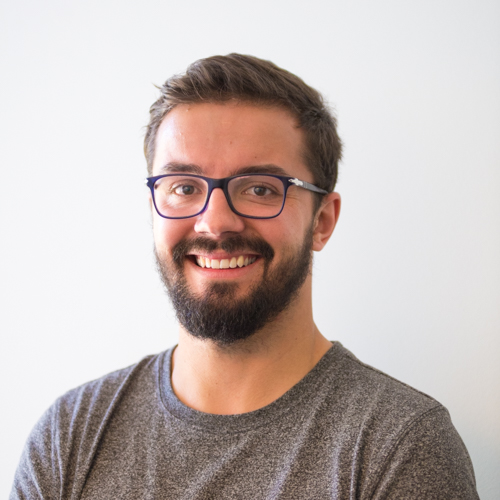
\includegraphics[width=\linewidth]{robertColour.jpg}	%trimming relative to image size

\cvsection{CONTACT}
	
\icontext{MapMarker}{12}{8/192-198 Princes Hwy\\Fairy Meadow, NSW 2519\\AUSTRALIA}{black}\\[6pt]
\icontext{MobilePhone}{12}{+61 433 614 163}{black}\\[6pt]
\iconemail{Envelope}{12}{robbie.mardus@gmail.com}{robbie.mardus@gmail.com}{black}\\[6pt]


%---------------------------------------------------------------------------------------
%	META SKILLS
%----------------------------------------------------------------------------------------
\cvsection{SKILLS}

\cvskill{Numerical Modelling} {5+ yrs} {1} \\[-2pt]

\cvskill {Linux} {5+ yrs} {1} \\[-2pt]

\cvskill{Open Source Tools} {4+ yrs} {0.8} \\[-2pt]

\cvskill{OpenFOAM} {4+ yrs} {0.8} \\[-2pt]

\cvskill{Monte Carlo Transport} {3+ yrs} {0.6} \\[-2pt]

\cvskill{C++} {3+ yrs} {0.6} \\[-2pt]

\cvskill{Python} {3+ yrs} {0.6} \\[-2pt]

\cvskill{git} {3+ yrs} {0.6} \\[-2pt]

\cvskill{SysAdmin} {2+ yrs} {0.4} \\[-2pt]

%\vfill\null

%\vfill\null
\qrcodelinkedin{0.65}

%---------------------------------------------------------------------------------------
%	EDUCATION
%----------------------------------------------------------------------------------------
\newpage
\cvsection{EDUCATION}

\cvmetaeventthreeline
{2016 - 2020}
{PhD. Engineering (Nuclear)}
{University of New South Wales}

\cvmetaeventthreeline
{2017-2018}
{Research Secondment}
{University of California,\newline Berkeley}

\cvmetaeventthreeline
{2010 - 2015}
{B. Engineering (Mechanical)\newline 1st Class Honours}
{University of Wollongong}

\cvmetaeventthreeline
{2010 - 2015}
{B. Science (Physics)\newline with Distinction }
{University of Wollongong}

\cvmetaeventthreeline
{2013}
{Student Exchange}
{University of Victoria,\newline British Columbia}

%---------------------------------------------------------------------------------------
%	CERTIFICATION
%----------------------------------------------------------------------------------------
\cvsection{CERTIFICATIONS}

\cvmetaevent
{CSIRO ON Prime}
{}
{}
{Part-time training in product and market development for start-ups concerned with novel products and services. Conducted as co-founder of Ouranos Systems.}

\cvmetaevent
{Online Classes}
{}
{}
{As part of my desire to become more competent at programming and progress my skills it is important that I keep extending my knowledge via taking online classes.}

\vfill\null
\qrcodeemail{0.65}

%\cvsection{AWARDS}

%\cvmetaevent
%{Business Engagement Scholarship}
%{}
%{}
%{Awarded as an initiative by NSW Government to encourage collaboration between research and business, and enable products to be brought to market.}

%\cvmetaevent
%{United Uranium Scholarship}
%{}
%{}
%{Awarded to attend conference and workshop as part of PhD research.}

%\cvmetaevent
%{Postgraduate Research Award}
%{}
%{}
%{}

%\vfill
%\qrcodeinstagram{0.65}

%\newpage
%--------------------------------------------
%   References
%--------------------------------------------
\cvsection{References}

\cvmetaeventthreeline
{Prof. Guan Yeoh}
{PhD Supervisor}
{g.yeoh@unsw.edu.au\newline +61 2 9385 4099}


\cvmetaeventthreeline
{Dr. Mark Ho}
{XX}
{mho@ansto.gov.au\newline 04XX XXX XXX}

\cvmetaeventthreeline
{Dr. Weijian Lu}
{Supervisor within Nuclear Analysis Section, ANSTO}
{XX@ansto.gov.au}

\cvmetaeventthreeline
{Mr. Adrian Purnell}
{Supervisor within Northrops Consulting Engineers}
{XX@northrops.com.au}



\end{leftcolumn}
\begin{rightcolumn}
%---------------------------------------------------------------------------------------
%	TITLE  HEADER
%----------------------------------------------------------------------------------------
\fcolorbox{white}{darkcol}{\begin{minipage}[c][3.5cm][c]{1\mpwidth}
	\begin {center}
		\LARGE{ \textbf{ \textcolor{white}{ \uppercase{ ROBERT MARDUS-HALL } } } } \\[-10pt]
		\textcolor{white}{ \rule{0.1\textwidth}{1.25pt} } \\[4pt]
		\large{ \textcolor{white} {Multiphysics Analyst and Engineering Consultant} }
	\end {center}
\end{minipage}} \\[14pt]
\vspace{-12pt}

%---------------------------------------------------------------------------------------
%	PROFILE
%----------------------------------------------------------------------------------------
\vfill\null
\cvsection{PROFILE}

\cvtext{Mechanical/Nuclear Engineer with skills in numerical simulation and a passion for OpenSource software.\\

}

%---------------------------------------------------------------------------------------
%	WORK EXPERIENCE
%----------------------------------------------------------------------------------------
\vfill\null
\cvsection{WORK EXPERIENCE}

\vfill\null
\cvevent
	{Mar 20 - NOW}
	{Multiphysics analyst}
	{Nuclear Analysis Section, ANSTO}
	{Responsible for}
	{\cvlist{
		\item 
	}}
	{\cvlist {
		\item StarCCM+
		\item SolidWorks
		\item 
	}}
	{\cvlist{
		\item Driving force behind procurement and implementation of modern hardware within section
		\item Design of novel Cold Neutron Source for future placement in thermal neutron guide
	}}
	
\vfill\null
\cvevent
	{Dec 19 - NOW}
	{Co-founder, Technical Officer}
	{Ouranos Systems Pty Ltd}
	{Responsible for}
	{\cvlist{
		\item 
	}}
	{\cvlist {
		\item Neutronics (Serpent, MCNP)
	}}
	{\cvlist{
		\item 
	}}

\vfill\null
\cvevent
	{Mar 17 - NOW}
	{System Administrator}
	{ARC Fire Safety Training Centre}
	{}
	{\cvlist{
		\item 
	}}
	{\cvlist {
		\item Standard Linux tools, such as htop, sed, grep, awk, ...
		\item 
	}}
	{\cvlist{
		\item 
	}}

\vfill\null
\cvevent
	{Mar 16 - Feb 20}
	{PhD Candidate}
	{University of New South Wales}
	{Independently researched and developed}
	{\cvlist{
		\item 
	}}
	{\cvlist {
		\item Standard Linux tools, such as htop, sed, grep, awk, ...
		\item Python for in-depth data analysis
	}}
	{\cvlist{
		\item 
	}}
	
\vfill\null
\cvevent
	{Mar 16 - Feb 19}
	{Head Tutor}
	{University of New South Wales, School of Mechanical and Manufacturing Engineering}
	{Independently researched and developed}
	{\cvlist{
		\item 
	}}
	{\cvlist {
		\item Standard Linux tools, such as htop, sed, grep, awk, ...
		\item Python for in-depth data analysis
	}}
	{\cvlist{
		\item 
	}}

\vfill\null
\cvevent
	{Dec 14 - Feb 15\newline Dec 15 - Feb 16}
	{Mechanical Engineer - Internship}
	{Northrop Consulting Engineers}
	{Independently researched and developed}
	{\cvlist{
		\item 
	}}
	{\cvlist {
		\item 
	}}
	{\cvlist{
		\item 
	}}


\vfill\null
\cvsection{AWARDS}

\cvtext{

\cvmetaevent
{Business Engagement Scholarship}
{}
{}
{Awarded as an initiative by NSW Government to encourage collaboration between research and business, and enable products to be brought to market.}

\cvmetaevent
{United Uranium Scholarship}
{}
{}
{Awarded to attend conference and workshop as part of PhD research.}

\cvmetaevent
{Postgraduate Research Award}
{}
{}
{}
}

% hotfixes to create fake-space to ensure the whole height is used
\mbox{}
\vfill
\mbox{}
\vfill
\mbox{}
\vfill
\mbox{}
\end{rightcolumn}
\end{paracol}
\end{document}

